\documentclass[../TinyBot.tex]{subfiles}
\begin{document}
    
\section{Motor Controller} \label{sec:motorcontroller}

The motors used in this guide, the N20 motors, have a stall current of 1.6A (see section \ref{sec:motor} for what stall current means). The digital pins on an Arduino Uno supply at most 40mA. This is not enough to power the motors.\\ 

To get around this, the Arduino instead interfaces with a \textbf{motor controller}. Motor controllers have a separate power supply that can supply enough current to drive the motor. Motor controllers also have digital inputs that allow control of the motor. \\


An added benefit of using a motor controller is that it is possible to control the direction and the speed of the motor. 

\bigskip

The phrase motor controller is often used as a generic term for any device, circuit, or IC which controls a motor. However, motor controllers are a circuit that consists of a motor driver and some digital harness that acts as an interface to the driver. Motor controllers can be dropped into a circuit and easily controlled, allowing feedback from the motor and more control than a simple driver provides. \\


% An example of a motor driver versus a motor controller is the \href{https://www.altronics.com.au/p/z2900-l293d-motor-drive-ic/}{L293D} motor driver versus the \href{https://www.altronics.com.au/p/z6442-l298n-dual-h-bridge-motor-module-for-arduino/}{L298N}. 


\subsection{Motor Driver}
A basic motor-\textbf{driver} is a H-bridge. The simplest H-bridge is shown in the below schematics, as well as an explanation of how using a H-bridge allows control over the motors direction. 

\begin{center}
    \begin{circuitikz}
    \draw (0,2) -- (0,0) to
        (0,0) to[nos, l^=$1$] (2,0) to
        (2,0) to [nos, l^=$2$] (4,0) to
        (4,0) -- (4,2) to
        (4,2) to[nos, l^=$3$] (2,2) to
        (2,2) to[nos, l^=$4$] (0,2);
    \draw (2,1) node[elmech](motor){M};
    \draw (motor.north) -- (2,2);
    \draw (motor.south) -- (2,0);
    \draw (0,1) -- (-1,1) node[vee]{};
    \draw (4,1) -- (5,1) node[ground]{};
    % \draw (2,0) to[sV, color=white, name=M] (2,2);
    % \mymotor{M}{90};
    % \draw[rotate=2] (0,2) \mymotor{M}{90} (2,2);
    \end{circuitikz}
    % \captionof{figure}{}
\end{center}
\bigskip

When switches $1$ and $3$ are closed, the current will flow through the motor making it turn anticlockwise.
% in the motor will flow in one direction. 

\begin{center}
    \begin{circuitikz}
        \draw (0,2) -- (0,0) to
            % (0,0) to[o-o, l_=$1$] (2,0) to
            (0,0) -- node[above, yshift=1.5mm]{1} (2,0) to
            (2,0) to [nos, l^=$2$] (4,0) to
            (4,0) -- (4,2) to
            % (4,2) to[l_=$3$] (2,2) to
            (4,2) -- node[below, yshift=-1.5mm]{3} (2,2) to
            (2,2) to[nos, l^=$4$] (0,2);
        \draw (motor.north) -- (2,2);
        \draw (motor.south) -- (2,0);
        \draw[color=red!100, thick] (0,1) -- (-1,1) node[vee]{};
        \draw[color=red!100, thick] (4,1) -- (5,1) node[ground]{};
     
        \begin{scope}[>=latex]
            \draw[->, color=red!100, thick] (-1,1) -- (0,1);
            \draw[->, color=red!100, thick] (0,1) -- (0,0);
            \draw[->, color=red!100, thick] (0,0) -- (2,0);
            \draw[->, color=red!100, thick] (2,0) -- (2,2);
            \draw[->, color=red!100, thick] (2,2) -- (4,2); 
            \draw[->, color=red!100, thick] (4,2) -- (4,1);
        \end{scope}
        \draw (2,1) node[elmech](motor){M};
        \centerarc[->](2,1)(-45:45:0.7);
        \centerarc[->](2,1)(135:225:0.7);
    \end{circuitikz}
\end{center}
\bigskip

In the same vein, closing switches 2 and 4 will cause the motor to turn clockwise. 
\begin{center}
    \begin{circuitikz}
        \draw (0,2) -- (0,0) to
            (0,0) to[nos, l^=$1$] (2,0) to
            % (2,0) to [nos, l_=$2$] (4,0) to
            (2,0) -- node[above, yshift=1.5mm]{2}(4,0) to 
            (4,0) -- (4,2) to
            (4,2) to[nos, l^=$3$] (2,2) to
            % (2,2) to[nos, l_=$4$] (0,2);
            (2,2) -- node[below, yshift=-1.5mm]{4} (0,2);
        \draw (motor.north) -- (2,2);
        \draw (motor.south) -- (2,0);
        \draw[color=red!100, thick] (0,1) -- (-1,1) node[vee]{};
        \draw[color=red!100, thick] (4,1) -- (5,1) node[ground]{};

        \begin{scope}[>=latex]
            \draw[->, color=red!100, thick] (-1,1) -- (0,1);
            \draw[->, color=red!100, thick] (0,1) -- (0,2);
            \draw[->, color=red!100, thick] (0,2) -- (2,2);
            \draw[->, color=red!100, thick] (2,2) -- (2,0);
            \draw[->, color=red!100, thick] (2,0) -- (4,0); 
            \draw[->, color=red!100, thick] (4,0) -- (4,1);
        \end{scope}
        \draw (2,1) node[elmech](motor){M};

        \centerarc[->](2,1)(45:-45:0.7);
        \centerarc[->](2,1)(225:135:0.7);

    \end{circuitikz}
\end{center}
\bigskip

If pins 4 \& 3 or pins 1 \& 2 are closed at the same time, a short circuit will be formed and the H-bridge will break. \\

\begin{minipage}{0.5\textwidth}\vspace{0pt}
    \begin{center}
        \begin{circuitikz}
            \draw (0,2) -- (0,0) to
                (0,0) to[nos, l^=$1$] (2,0) to
                (2,0) to [nos, l^=$2$] (4,0) to
                % (2,0) -- node[below, yshift=-1.5mm]{2}(4,0) to 
                (4,0) -- (4,2) to
                % (4,2) to[nos, l_=$3$] (2,2) to
                % (2,2) to[nos, l_=$4$] (0,2);
                (4,2) -- node[below, yshift=-1.5mm]{3} (2,2) to
                (2,2) -- node[below, yshift=-1.5mm]{4} (0,2);
            \draw (motor.north) -- (2,2);
            \draw (motor.south) -- (2,0);
            \draw[color=red!100, thick] (0,1) -- (-1,1) node[vee]{};
            \draw[color=red!100, thick] (4,1) -- (5,1) node[ground]{};
            
            \begin{scope}[>=latex]
                \draw[->, color=red!100, thick] (-1,1) -- (0,1);
                \draw[->, color=red!100, thick] (0,1) -- (0,2);
                \draw[->, color=red!100, thick] (0,2) -- (2.1,2);
                \draw[->, color=red!100, thick] (2,2) -- (4.01,2);
                % \draw[->, color=red!100, thick] (2,0) -- (4,0); 
                \draw[->, color=red!100, thick] (4,2) -- (4,1);
            \end{scope}
            \draw (2,1) node[elmech](motor){M};
    
        \end{circuitikz}
    \end{center}
\bigskip

\end{minipage}
\begin{minipage}{0.5\textwidth}\vspace{0pt}
    \begin{center}
        \begin{circuitikz}
            \draw (0,2) -- (0,0) to
                % (0,0) to[nos, l_=$1$] (2,0) to
                % (2,0) to [nos, l_=$2$] (4,0) to
                (0,0) -- node[above, yshift=1.5mm]{1}(2,0) to 
                (2,0) -- node[above, yshift=1.5mm]{2}(4,0) to 
                (4,0) -- (4,2) to
                (4,2) to[nos, l^=$3$] (2,2) to
                (2,2) to[nos, l^=$4$] (0,2);
                % (2,2) -- node[above, yshift=1.5mm]{4} (0,2);
            \draw (motor.north) -- (2,2);
            \draw (motor.south) -- (2,0);
            \draw[color=red!100, thick] (0,1) -- (-1,1) node[vee]{};
            \draw[color=red!100, thick] (4,1) -- (5,1) node[ground]{};    
    
            \begin{scope}[>=latex]
                \draw[->, color=red!100, thick] (-1,1) -- (0,1);
                \draw[->, color=red!100, thick] (0,1) -- (0,0);
                \draw[->, color=red!100, thick] (0,0) -- (2.1,0);
                % \draw[->, color=red!100, thick] (2,2) -- (2,0);
                \draw[->, color=red!100, thick] (2,0) -- (4,0); 
                \draw[->, color=red!100, thick] (4,0) -- (4,1);
            \end{scope}
            \draw (2,1) node[elmech](motor){M};
    
        \end{circuitikz}
    \end{center}
\end{minipage}

\bigskip \bigskip

Breaking a H-bridge is fairly common, especially the cheaper low power ones. Some higher end H-bridges are designed to prevent the H-bridge from shorting if the wrong pins are closed. 
Most motor-controllers will have this protection built-in, though most motor-drivers do not.


While working on this guide, don't worry if your H-bridge stops working suddenly, it is quite common to short them out. 

\bigskip


% In the case of the H-bridge, the voltage supplied (from the left on the diagrams displayed above) is a high enough voltage, with a high enough current, to drive the motor. The switches (1, 2, 3, 4) are, in their simplest form, a button that is closed upon a signal from the microcontroller. Switches require a very small amount of power to close, and so can be controlled directly from the motor controller. 



\subsection{Motor Controller}
% https://www.robotshop.com/en/roboclaw-2x30a-6-34vdc-regenerative-motor-controller.html

\begin{minipage}{0.3\textwidth}\vspace{0pt}
    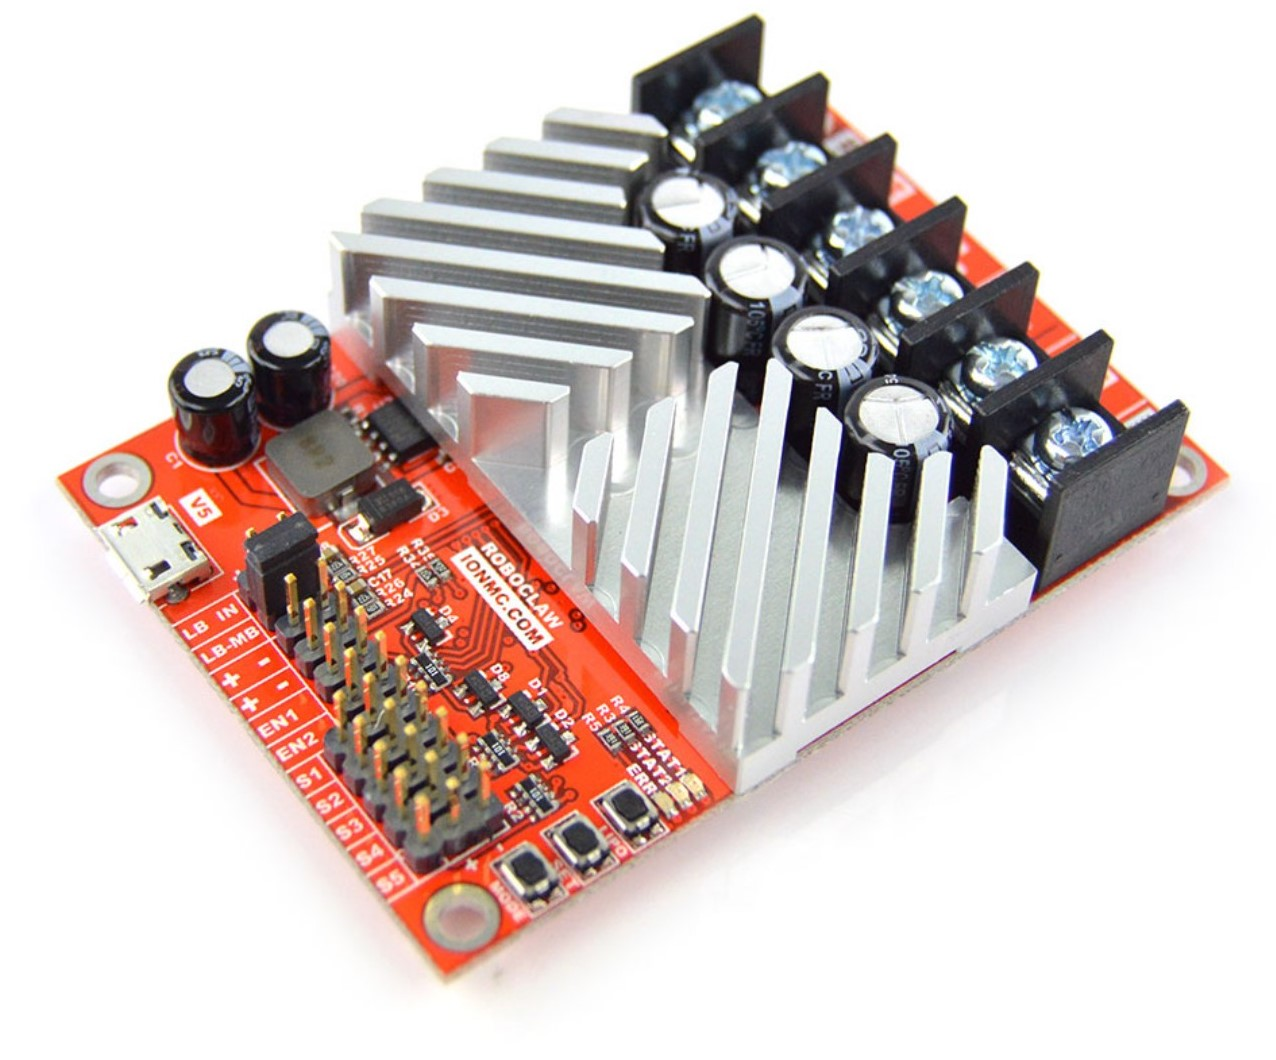
\includegraphics[width=\textwidth]{roboclaw.jpg}
    \captionof{figure}{\href{https://www.robotshop.com/media/files/content/b/bat/pdf/roboclaw_datasheet_2x30a-2.pdf}{RoboClaw Motor Controller}}
    \label{fig:roboclaw}
\end{minipage}
\begin{minipage}{0.7\textwidth}\vspace{0pt}
    A motor controller has a lot more features than a motor driver. See, for example, the RoboClaw  (see Figure \ref{fig:roboclaw}) which has in built features such as PID tuning, data logging, diagnostic LEDs, and serial control. \\
    
    
    The in-built control modes, as well as being capable of serial communication, is present only in motor controllers. Motor drivers are far simpler in comparison. \\

\end{minipage}

\pagebreak
\subsection{L293D H-Bridge IC}

The information in this section is included for information's sake, you don't need to understand it to be able to build TinyBot; though it can be useful knowledge. You can skip this section if you would like. \\



Datasheets hold a lot of useful information about microchips, the data sheet for the L293D H-Bridge can can be found online (linked \href{https://www.altronics.com.au/p/z2900-l293d-motor-drive-ic/}{here}).\\



\begin{center}
    \centering

    \begin{minipage}{0.5\textwidth}\vspace{0pt}
        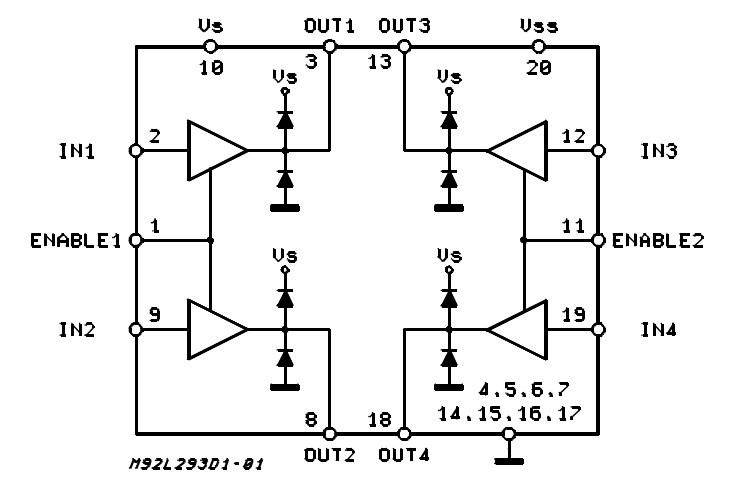
\includegraphics[width=\textwidth]{L293D-block-diagram.jpg}
        \caption{Block Diagram for 20 Pin Chip}
        \label{fig:l293d-block-diagram}
        
    \end{minipage}
    \begin{minipage}{0.2\textwidth}\vspace{0pt}
        
    \end{minipage}
    \begin{minipage}{0.3\textwidth}\vspace{0pt}
        \centering
        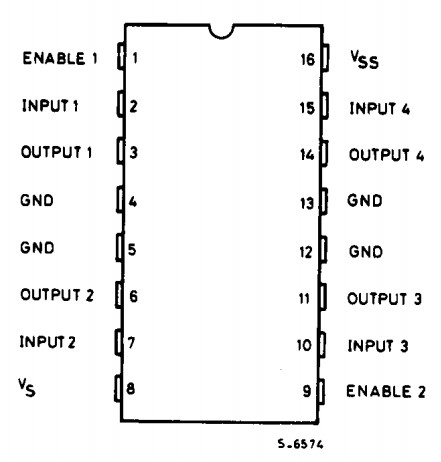
\includegraphics[width=\textwidth]{L293D-pinout.jpg}
        \caption{Pinout of 16 Pin Chip}
        \label{fig:l293d-pinout}
    \end{subfigure}
    \caption{Diagrams from the L293D datasheet}
    \label{fig:l293d}
\end{center}

\FloatBarrier


Being able to read diagrams such as in Figure \ref{fig:l293d-block-diagram} really depends on whether or not you know what each symbol means. \\

% Block diagrams such as in Figure \ref{fig:l293d-block-diagram} can be quite confusing to read; there's a lot of symbols that you may or may not know. 

The hollow circles along the outside rectangle of the block diagram represent the pin outs on the microchip, they can be matched up with labelled pins in Figure \ref{fig:l293d-pinout}. There is also a 20 pin variant of this H-bridge, which is why some of the pin labels on the block diagram are greater than 16.\\


The hollow triangles in the block diagram are buffers that isolate the the input signal from the enable line. \\



The bold black triangle and line combinations represent components called Transistors. 




% MOSFETs. They essentially work as electric switches; providing the right signal to the MOSFET will allow current to flow in much the same manner as pressing a push buttons allows current to flow as shown in Figure \ref{fig:mosfet-conceptual}.

% \begin{center}
    
%     \begin{tikzpicture}[scale=0.5]
%         \filldraw (0,3) circle (2pt) node[align=left, left] {\lstinline[]!ENABLE1!} -- (2,3);
%         \draw (2,4) -- (4,4);
%         \filldraw (3,5) circle (2pt) node[align=center, above] {\lstinline[]!IN1=LOW!}-- (3,4);
%         \filldraw (6,3) circle (2pt) node[align=right, right] {\lstinline[]!OUT1!} -- (4,3);
        
%         \filldraw (0,0) circle (2pt) node[left] {\lstinline[]!ENABLE1!} -- (6,0) circle (2pt) node[right] {\lstinline[]!OUT1!};
%         \filldraw (3,1) circle (2pt) node[above] {\lstinline[]!IN1=HIGH!} -- (3,0);
%     \end{tikzpicture}
%     \captionof{figure}{MOSFET}
%     \label{fig:mosfet-conceptual}
% \end{center}
% A MOSFET is an advanced digital component, not discussed in University till about 3rd year engineering units. This information about MOSFETs is included for completeness, and to satisfy any curiosity. It is not important to understand MOSFETs at this level, though if you are curious the internet has many resources available for learning about electrical components in depth which act as the switches in the circuit. \\

% % (depicted as the bold black triangle and lines, they are the "switches" in this H-Bridge). Basically, setting \lstinline[]!IN1=HIGH! when \lstinline[]!ENABLE1=HIGH! will close the switch and provide power to \lstinline[]!OUT1!. 

% % Using the buffer allows a low voltage signal, from the digital ports on the Arduino, to close the switch while using the higher voltage from \lstinline[]!ENABLE1! to flow through and power the motor. 

% % % It can be thought of as 

% % If \lstinline[]!ENABLE! has no power, then the motor will not turn; the voltage provided from the digital pins is not sufficient to drive the motor.  This is why in the wiring diagram (Figure \ref{fig:schematic-hbridge}) you'll notice that all 4 \lstinline[]!ENABLE! pins are all linked and permanently set to 9V (\lstinline[]!HIGH!) \\





\end{document}